\documentclass{beamer}
\usetheme{Boadilla}

\usepackage{amsmath}
\usepackage{amsfonts}
\usepackage{hyperref}
\usepackage{amsthm}



\title{Dual form of SGD via Attention}
\author{Skorik Sergey}
\institute{MIPT, 2022}


\begin{document}

\begin{frame}
    \titlepage
\end{frame}


\begin{frame}
    \tableofcontents
\end{frame}

\section{Preliminaries}

\begin{frame}{Motivation}

    \begin{block}{Introduction}
Despite the broad success of neural nets (NNs) in many applications, much of their internal functioning remains obscure. Naive visualisation of their activations or weight matrices rarely shows human-interpretable patterns. In this paper authors propose to revisit the dual form of the perceptron (Aizerman et al., 1964) and apply it in the modern context of deep NNs, with the objective of better understanding how training datapoints relate to test time predictions in NNs.
    \end{block}
\end{frame}

\begin{frame}{Preliminaries}
    \begin{block}{Attention}
        \textbf{Definition}(Unnormalized Dot Attention) let $\mathbf{K} = (\mathbf{k}_1, \ldots \mathbf{k}_T) \in \mathbb{R}^{d_{\text{in}}\times T}$ and $\mathbf{V} = (\mathbf{v}_1, \ldots \mathbf{v}_T) \in \mathbb{R}^{d_{\text{out}}\times T}$ denote matrices representing $T$ key and value vectors. Let $\mathbf{q} \in \mathbb{R}^{d_{\text{in}}}$ denote a query vector. An unnormalised linear dot attention operation $Attention(\mathbf{K}, \mathbf{V}, \mathbf{q})$ computes the following weighted average of value vectors $\mathbf{v}_t$:
        \begin{equation}\label{def_attn}
            Attention(\mathbf{K}, \mathbf{V}, \mathbf{q}) = \sum_{t=1}^T\alpha_t\mathbf{v}_t
        \end{equation}
        where the weights $\alpha_t = \mathbf{k}^\top_t \mathbf{q} \in \mathbb{R}$ are dot products between key $\mathbf{k}_t $ and query $\mathbf{q}$ vectors, and are called attention weights. 
    \end{block}
\end{frame}

\begin{frame}{Preliminaries}
    \begin{figure}[h]
    \centering
    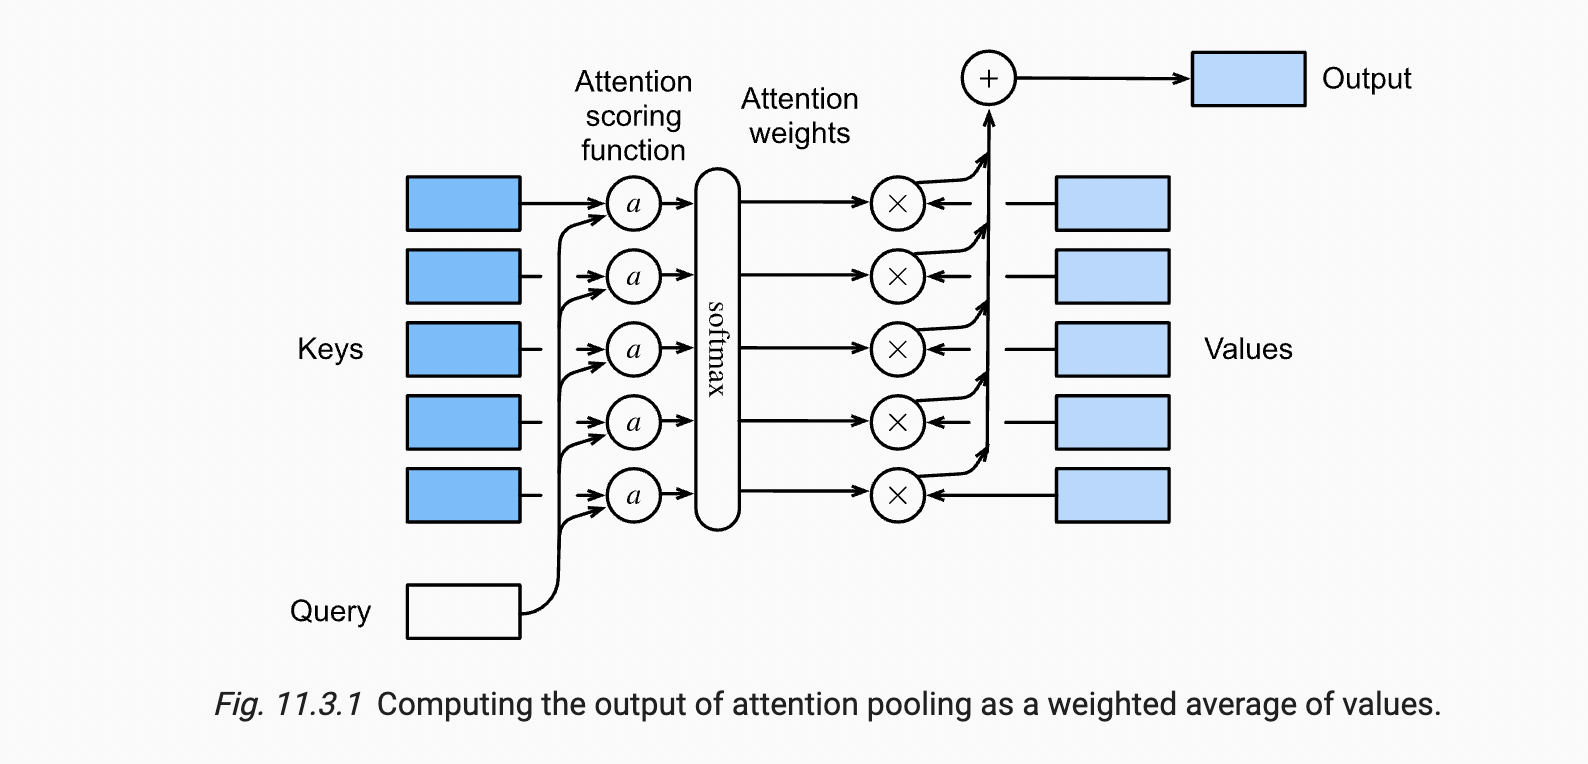
\includegraphics[width=10cm, height=5cm]{attention_model.png}
\end{figure}
\end{frame}

\begin{frame}{Preliminaries}
    \begin{block}{Matrix form}
        \textbf{Corollary}: Attention computation defined above can be expressed as:
        \begin{equation}\label{mf_attn}
            Attention(\mathbf{K}, \mathbf{V}, \mathbf{q}) = \mathbf{V}\mathbf{K}^\top\mathbf{q}
        \end{equation}
        \textit{Proof}:
        \begin{equation*}
            Attention(\mathbf{K}, \mathbf{V}, \mathbf{q}) = \sum_{t=1}^T\alpha_t\mathbf{v}_t = \sum_{t=1}^T\mathbf{v}_t\alpha_t = \sum_{t=1}^T\mathbf{v}_t\mathbf{k}^\top_t \mathbf{q} = \left(\sum_{t=1}^T\mathbf{v}_t\mathbf{k}^\top_t\right) \mathbf{q}
        \end{equation*}
    \end{block}
    \begin{block}{Equivalent System}
         Two systems $S_1$ and $S_2$ defined over the same input and output domains $\mathcal{D}_{in}$ and $\mathcal{D}_{out}$, are said to be \textit{equivalent} if and only if for any input, their outputs are equal, i.e., for any $\mathbf{x} \in \mathcal{D}_in$, the following holds
         \begin{equation}\label{def_eqsys}
             S_1(\mathbf{x}) = S_2(\mathbf{x})
         \end{equation}
    \end{block}
\end{frame}

\section{The main idea}

\begin{frame}{Idea}
    \begin{figure}[t]
        \centering
        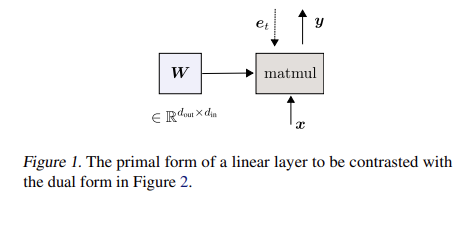
\includegraphics[width=6cm, height=3cm]{LNN_primal.png}
    \end{figure}
    \begin{figure}[b]
        \centering
        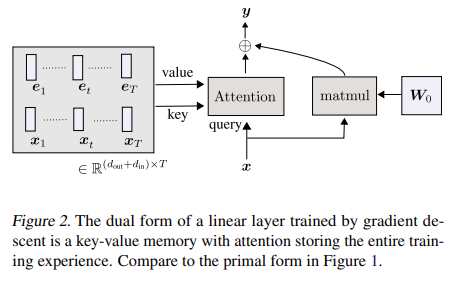
\includegraphics[width=6cm, height=3cm]{Attn_dual.png}
    \end{figure}
\end{frame}

\begin{frame}{Duality}
    \begin{block}{Corollary}
        The following systems $S_1$, $S_2$ are equivalent:
        \begin{itemize}
            \item $S_1$ (\textit{Primal form}): A linear layer in a neural network trained
        by gradient descent in some error function using T training
        inputs to this layer $(\mathbf{x}_1, \ldots, \mathbf{x}_T)$ with $\mathbf{x}_t \in \mathbb{R}^{d_{in}}$  and corresponding (backpropagation) error signal $(\mathbf{e}_1, \ldots, \mathbf{e}_T)$ with $\mathbf{e}_t \in \mathbb{R}^{d_{out}}$ obtained by gradient descent. Its weight matrix $\mathbf{W}\in\mathbb{R}^{d_{\text{in}}\times d_{\text{out}}}$  is thus:
        \begin{equation}\label{primal_backprop}
            \mathbf{W} = \mathbf{W}_0 + \sum_{t=1}^T \mathbf{e}_t \otimes \mathbf{x}_t
        \end{equation}
        Where $\mathbf{W}_0 \in \mathbb{R}^{d_{\text{in}}\times d_{\text{out}}}$ in is the initialisation. The layer transforms input $\mathbf{x}\inmathbb{R}^{d_{\text{in}}}$ to output $S_1(\mathbf{x})\in\mathbb{R}^{d_{\text{out}}}$ as:
        \begin{equation}\label{primal_form}
            S_1(\mathbf{x}) = \mathbf{W}\mathbf{x}
        \end{equation}
        \end{itemize}
    \end{block}
\end{frame}

\begin{block}{Corollary}
    \begin{itemize}
        \item $S_2$ (\textit{Dual form}):  A layer which stores T key-value pair $(\mathbf{x}_1, \mathbf{e}_1), \ldots (\mathbf{x}_T, \mathbf{e}_T)$ i.e., a key matrix $\mathbf{X} = (\mathbf{x}_1, \ldots, \mathbf{x}_T)\in\mathbb{R}^{d_{\text{in}}\times T}$ and a value matrix $\mathbf{E} = (\mathbf{e}_1, \ldots, \mathbf{e}_T)\in\mathbb{R}^{d_{\text{out}}\times T}$, and a weight matrix $\mathbf{W}_0 \in \mathbb{R}^{d_{\text{in}}\times d_{\text{out}}}$ which transforms input $\mathbf{x}\in\mathbb{R}^{d_{\text{in}}}$ to output $S_2(\mathbf{x})\in\mathbb{R}^{d_{\text{out}}}$ as:
        \begin{equation}\label{dual_form}
            S_2(\mathbf{x}) = \mathbf{W}_0\mathbf{x} + Attention(\mathbf{X}, \mathbf{E}, \mathbf{x})
        \end{equation}
    \end{itemize}
    \textit{Proof}:
    \begin{equation*}
        S_1(\mathbf{x}) = \mathbf{W}\mathbf{x} = \mathbf{W}_0\mathbf{x} + \sum_{t=1}^T \mathbf{e}_t \otimes \mathbf{x}_t\cdot\mathbf{x} = \mathbf{W}_0\mathbf{x} + Attention(\mathbf{X}, \mathbf{E}, \mathbf{x})
    \end{equation*}
\end{block}

\begin{frame}{Remarks}
    \begin{block}{Remark 1}
        \textbf{Nothing is "forgotten":}

        The entire life of an NN is recorded and stored as a key matrix X and value matrix E. Roughly speaking, the only limitation of the model’s capability to “remember” something is the limitation of the retrieval process
    \end{block}
    \begin{block}{Remark 2}
        \textbf{Unlimited memory size is not necessarily useful:}

        Systems which store everything in memory by increasing its size for each new event ($S_2$) are not necessarily better than those with a fixed size storage ($S_1$). 
    \end{block}
    \begin{block}{Remark 3}
        \textbf{Non-Uniqueness:}

        The expression of a linear layer as an attention system is not unique.
    \end{block}
\end{frame}

\section{Experiments}

\begin{frame}{Main Setup}
    \begin{block}{Common settings}
    \begin{equation*}
        Attention(\mathbf{X}, \mathbf{E}, \mathbf{x}) = \mathbf{E}\mathbf{X}^\top\mathbf{q} = \sum_{t=1}^T  \mathbf{x}_t\mathbf{x}\cdot\mathbf{e}_t = \sum_{t=1}^T\alpha_t\mathbf{e}_t
    \end{equation*}
        We posit that the dual formulation of linear layers offers a possibility to visualise how different training datapoints (i.e., a set of input/error signal pairs seen during training) contribute to some NN’s test time predictions.

        In the paper considering three different scenarios: single-task training, multi-task joint training, and multi-task continual training for image classification using feedforward NNs with two hidden layers. Analogous experiments also are conducted with language modelling using a one-layer LSTM recurrent NN.
    \end{block}
\end{frame}

\begin{block}{How to conduct the experiments?}
    \begin{itemize}
        \item Train a neural network using SGD and backprop.
        \item Save all $x_t$ and $e_t$ for each layer on each iteration.
        \item Take a test sample $\hat{\mathbf{x}}$, pass it through the neural network, get a test query and calculate $Attention(\mathbf{X}, \mathbf{E}, \hat{\mathbf{x}})$. 
    \end{itemize}
\end{block}

\begin{block}{Limitations}
    Since storing the inputs to each linear layer for the entire training experience can be highly demanding in terms of disk space, the authors works with small a datasets: MNIST, Fashion-MNIST (for image classification) and small domain book, WikiText-2 for language modelling. 
\end{block}

\begin{block}{Common model}
    Our model for image classification has two hidden layers with 800 nodes, each using relu activation functions after each layer. The total storage of training patterns is thus roughly $3\times800\times T$ units, where $T$ is the “number of training datapoints.
\end{block}

\begin{frame}{Single-Task Case}
    \begin{block}{Setup}
        The model is trained on MNIST dataset for $3K$ updates using a batch size of 128 which correspond to $384 K$-long training key/value memory slots. The resulting model achieves $97\%$ accuracy on the test set.
    \end{block}
    \begin{block}{How to interpreter attention weights?}
        \begin{itemize}
            \item Take test sample with some target $i=\overline{0, 9}$, run through all memory slots and get attention weights
            \item Sorting attention weights according to the training samples $\mathbf{x}_t$ classes.
            \item The resulting "groups" of weights are compared in two ways:
            \begin{itemize}
                \item \textbf{Attention weights distribution:} Get top 500 attention weights in each group by weight value
                \item \textbf{Total attention weights:} Sum attention weights in each group.
            \end{itemize}
        \end{itemize}
    \end{block}
\end{frame}

\begin{frame}
    \begin{figure}[h]
    \centering
    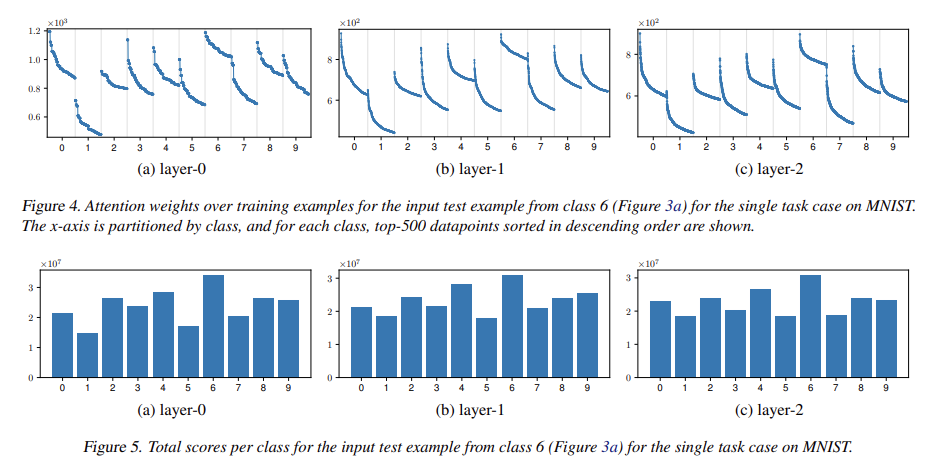
\includegraphics[width=11cm, height=8cm]{Single_task_sample.png}
\end{figure}
\end{frame}

\begin{frame}
\begin{figure}[h]
    \centering
    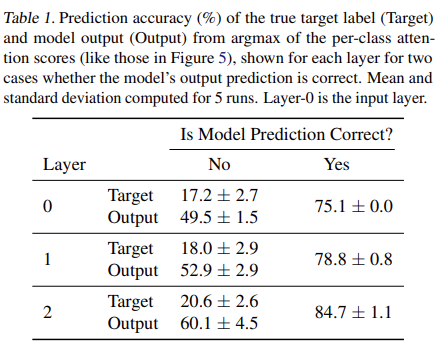
\includegraphics[width=6cm, height=6cm]{single_task_results.png}
\end{figure}
\end{frame}

\begin{frame}{Multi-Task Case}
    \begin{block}{Setup}
        The model is trained on MNIST and F-MNIST (at the same time) dataset for $5K$ updates and achieves $97\%$ and $87\%$ test accuracy on MNIST and F-MNIST, respectively. The output dimension remains 10, so, samples in other domain, but in the same targets are joined. using a batch size of 128 which correspond to $384 K$-long training key/value memory slots. The resulting model achieves $97\%$ accuracy on the test set.
    \end{block}
    \begin{block}{How to interpreter attention weights?}
        \begin{itemize}
            \item Calcluate attention weigths in the same manner as in Single-Task Case.
            \item In opposite to target classes, we split attention weigths into $20$ classes.
            \item The main observation in cross-task attention weights.
        \end{itemize}
    \end{block}
\end{frame}

\begin{frame}
\begin{figure}[h]
    \centering
    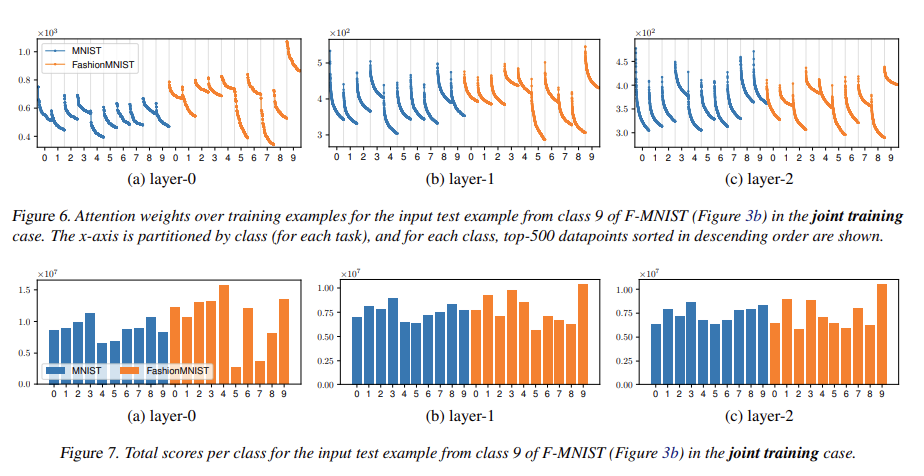
\includegraphics[width=11cm, height=8cm]{Multi_task_sample.png}
\end{figure}
\end{frame}

\begin{frame}{Continual Learning Case}
    \begin{block}{Setup}
    The model is trained on MNIST and F-MNIST subsequence:  first on MNIST for 3,000 steps,
then on F-MINST for 3,000 steps. The final test accuracies are $85\%$ on F-MNIST and $45\%$ on MNIST (down from $97\%$ after training on MNIST only).
    \end{block}
    \begin{block}{How to interpreter attention weights?}
        \begin{itemize}
            \item Calcluate attention weigths in the same manner as in Single-Task Case.
            \item Analogous to Multi-Task Case, we have $20$ classes of attention weights. 
            \item If we used an attention mask on the F-MNIST part of training keys for the attention computation, the model would be able to reproduce the good performance on MNIST obtained after the first part of training. 
        \end{itemize}
    \end{block}
\end{frame}

\begin{frame}
\begin{figure}[h]
    \centering
    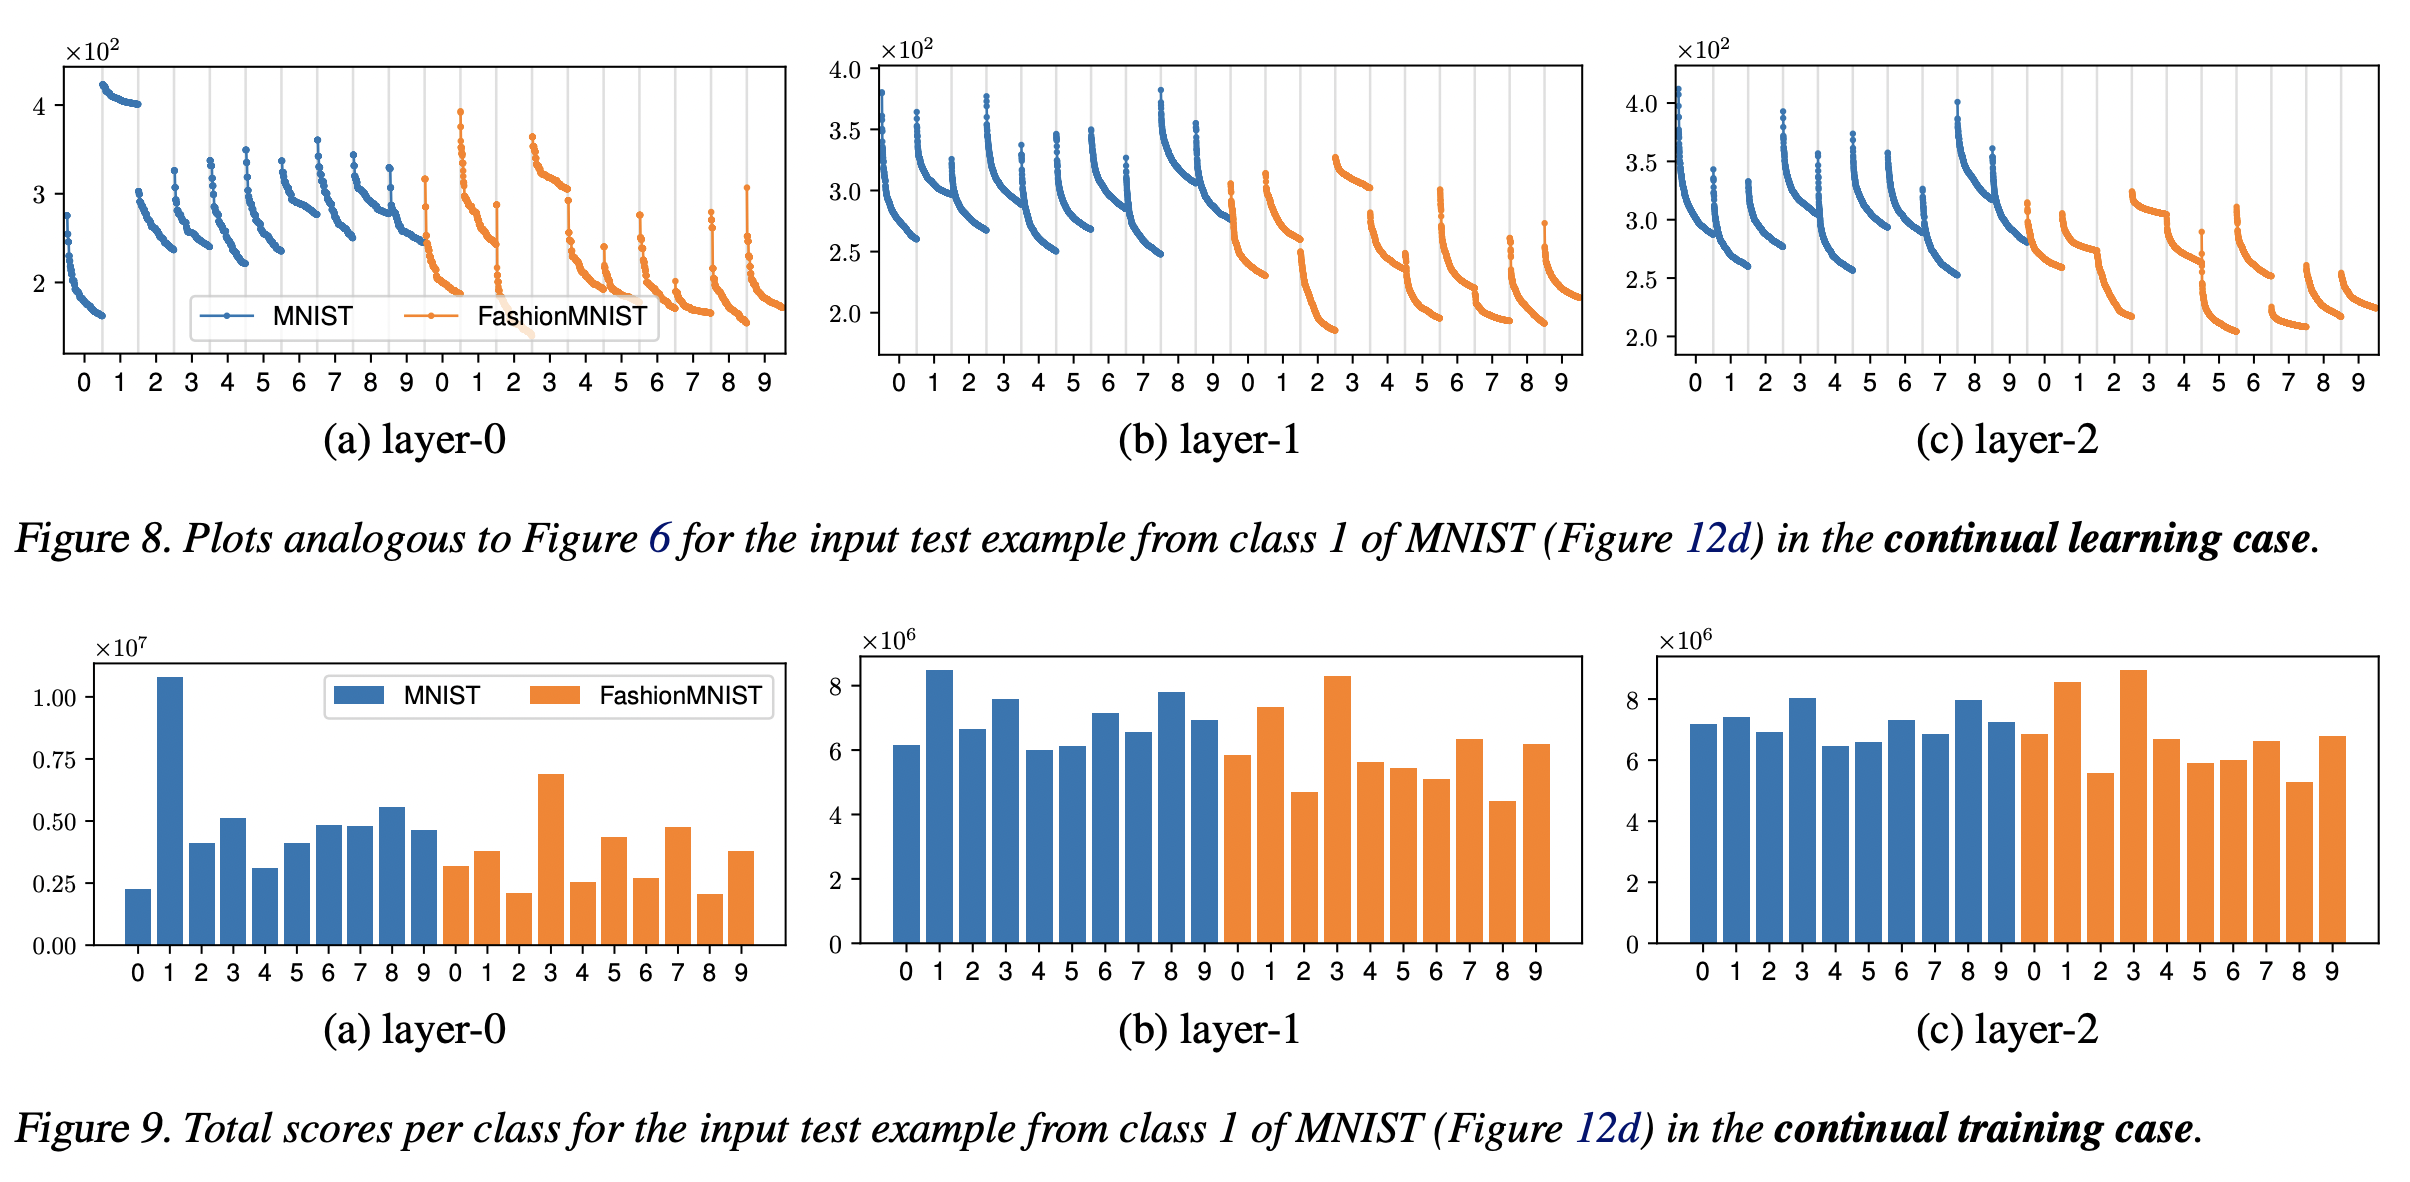
\includegraphics[width=11cm, height=9cm]{Continual_learning_sample.png}
\end{figure}    
\end{frame}

\begin{frame}{Language modelling}
    \begin{block}{Setup}
        In the experiment using one-layer LSTM LM on two small datasets: a tiny public domain book, “Aesop’s Fables”, by J. H. Stickney and the standard WikiText-2 dataset.
    \end{block}
    \begin{block}{How to interpreter attention weights?}
        \begin{itemize}
            \item Train LSTM, store inputs for each linear layer
            \item At test time, we forward the trained LM on a prompt (short text segment) and get the test query from the last token from the prompt.
            \item Grouping attention weights by training token position.
        \end{itemize}
    \end{block}
\end{frame}

\begin{frame}
    \begin{figure}[h]
    \centering
    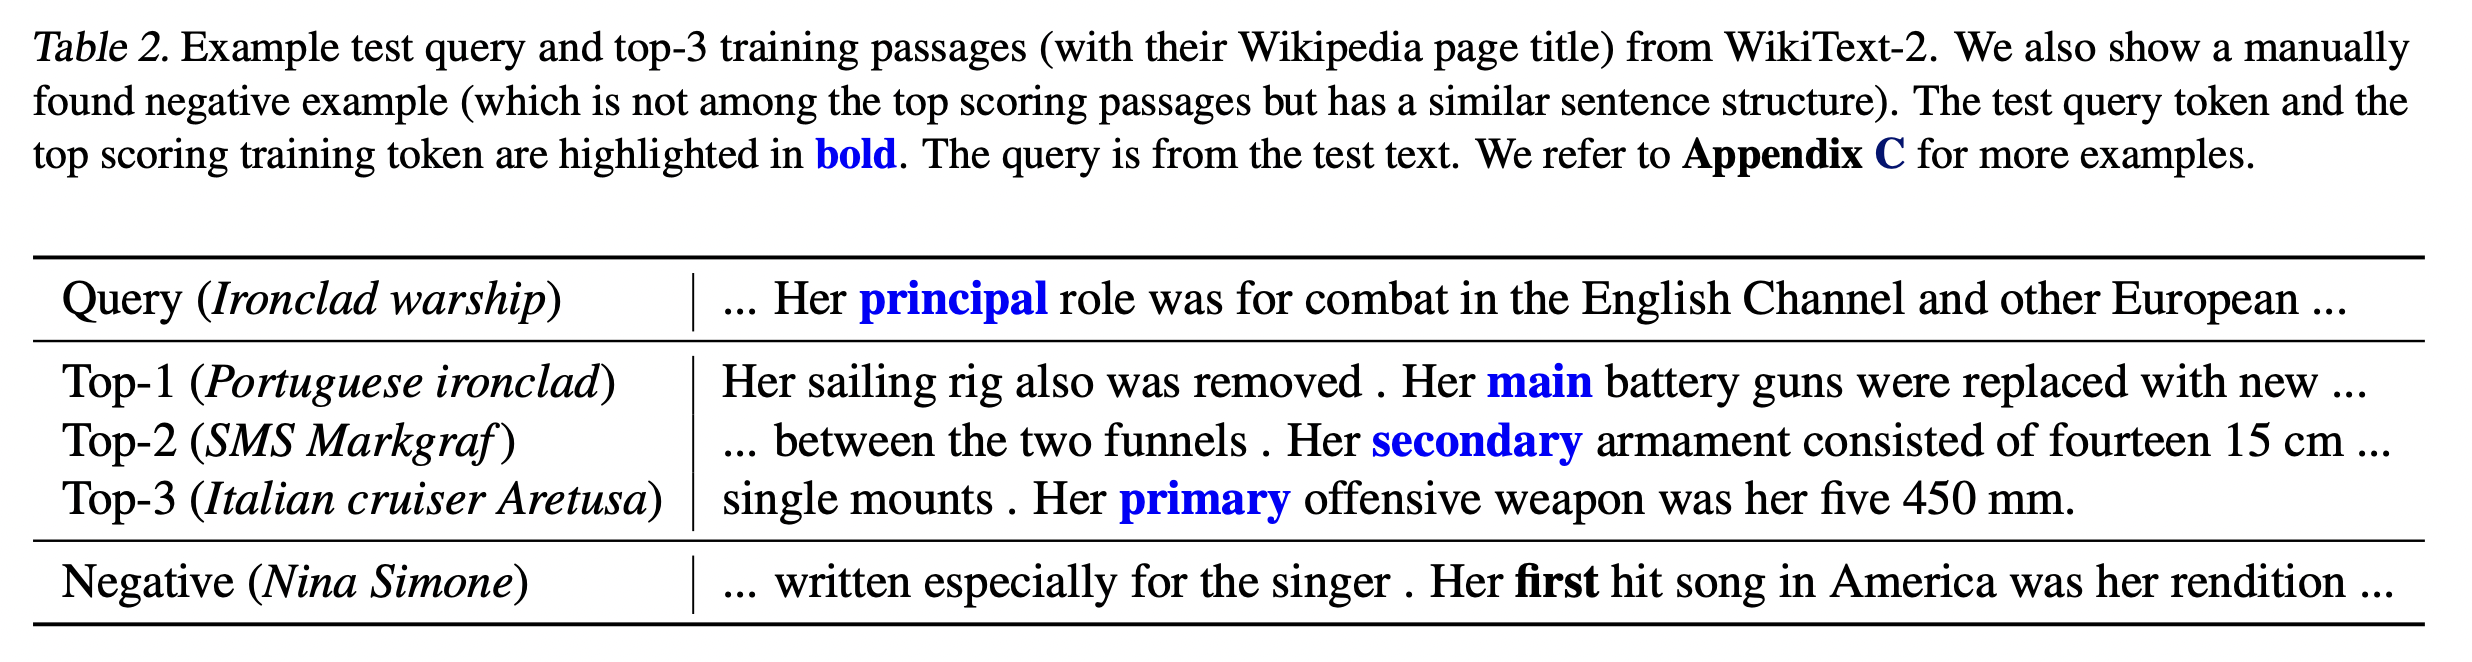
\includegraphics[width=11cm, height=4.5cm]{NLP_sample.png}
\end{figure} 
\end{frame}

\section{Discussion}

\begin{frame}{Discussion and Limitations}
    \begin{itemize}
        \item explicit visualization of attention weights. New point of view on NN's
        \item memory storage requirement
        \item analysis is not applicable to models which are already trained
        \item it is limited to a study of attention weights, in line with traditional visualisations of attention-based systems, and can only show which training datapoints are combined. It does not tell how the combined representations can be converted to a meaningful output, e.g., in the case of large generative NNs.
    \end{itemize}
\end{frame}

\end{document}